\documentclass[12pt]{beamer}

\usepackage[UTF8]{ctex}
\usepackage{bm}
\usepackage{cleveref}
\usepackage{hyperref}
\usetheme[progressbar=frametitle]{metropolis}



\begin{document}

\begin{frame}[allowframebreaks]{动态规划及其在路径规划中的作用}
         图的数学表示(存储方式)
         
         有向图最短路径问题的手工求解
         
         graphshortestpath函数
         
         Dijkstra算法
\end{frame}

\begin{frame}[allowframebreaks]{图的矩阵表示法}

关联矩阵:存储起点,终点和权值。

命令语句:

$a=[a_1,a_2,...,a_m,n];$起点

$b=[b_1,b_2,...,b_m,n];$终点

$w=[w_1,w_2,...,w_m,0];$权

$R=sparse(a,b,w);$关联矩阵的稀疏矩阵表示

\end{frame}

\begin{frame}[allowframebreaks]{最短路径问题手工求解}
例:求解1-9的最短路径
插图237页图6-16
\end{frame}
\begin{frame}[allowframebreaks]{有向图搜索及图示}
命令语句:

$P=biograph(R)$

$[d,p]=graphshortestpath(R,n_1,n_2)$,其中$n_1$为起点,$n_2$为终点。

例题解法:

$ab=[1 1 2 2 3 3 4 4 4 4 5 6 6 7 8];$

$bb=[2 3 5 4 4 6 5 7 8 6 7 8 9 9 9];$

$w=[1 2 12 6 3 4 4 15 7 2 7 7 15 3 10];$

R=sparse(ab,bb,w);建立关联矩阵

R(9,9)=0;

h=view(biograph(R,[],'ShowWeights','on'))显示有向图

[d,p]=graphshortestpath(R,1,9)计算最短路径,返回最短路径长度和路径节点
 
set(h.Nodes(p),'Color',[1 0 0])将路径节点标记成红色

\end{frame}

\begin{frame}[allowframebreaks]{有向图搜索及图示}
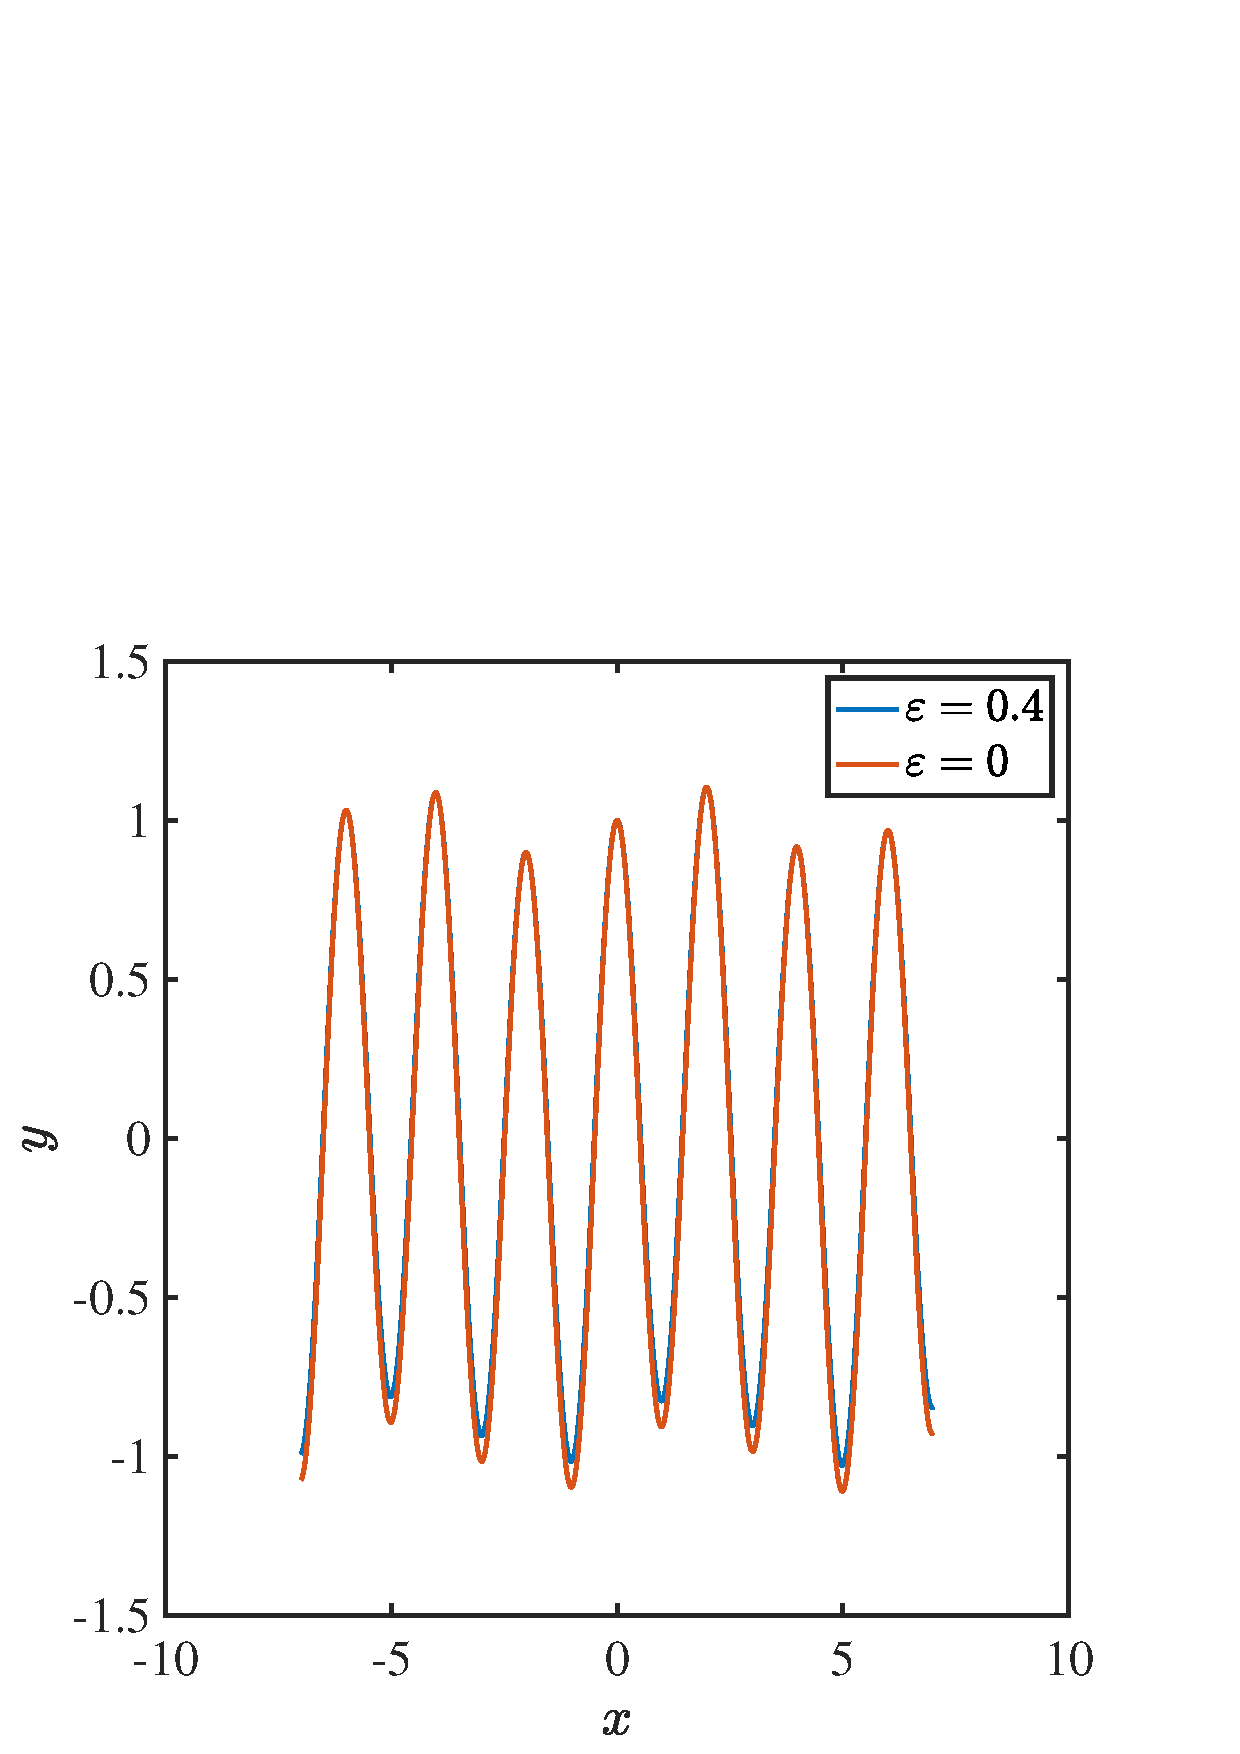
\includegraphics[width = 0.8\textwidth]{1.png}

\includegraphics[width = 0.8\textwidth]{2.png}

\end{frame}

\begin{frame}[allowframebreaks]{Dijkstra算法}
Dijkstra其人:

Edsger Wybe Dijkstra (04/01/1930-08/06/2002),  荷兰皇家艺术与科学学院的院士,美国科学院院士,英国计算协会的Fellow。年轻时代,Dijkstra在University of Leiden(荷兰最古老的大学)学习理论物理,但很快他就意识到其兴趣不在于理论物理虽然获得了其数学和理论物理的学位。

1984年至1999年,作为计算机系系主任任职与美国UT Austin(得克萨斯州大学奥斯汀分校),并于1999年退休。 
 
\includegraphics[width = 0.5\textwidth]{3.png}

E. W. Dijkstra 15年的学术著作覆盖了图论的理论工作,教育手册,解释文章和编程语言领域的哲学思考。

\end{frame}
\begin{frame}[allowframebreaks]{Dijkstra算法基本思路}
准备工作:

$\circ$设图G中有n个顶点,设置一个集合U存放已求出最短路径的顶点,V-U是尚未确定最短路径的顶点集合

$\circ$每个顶点对应一个距离值,则
集合U中顶点的距离值是从顶点v0到该顶点的最短路径长度;
集合V-U中顶点的距离值是从顶点v0到该顶点的只包括集合U中顶点为中间顶点的最短路径长度
\end{frame}
\begin{frame}[allowframebreaks]{Dijkstra算法基本思路}
初始状态:

$\circ$集合U中只有顶点v0,顶点v0对应的距离值为0

$\circ$集合V-U中顶点vi的距离值为边(v0,vi)的权值(i=1,…,n-1),如果v0和vi间无边直接相连,则vi的距离值为∞

在集合V-U中选择距离值最小的顶点vmin加入集合U

对集合V-U中各顶点的距离值进行修正,如果加入顶点vmin为中间顶点后,使v0到vi的距离值比原来的距离值更小,则修改vi的距离值

反复操作,直到从v0出发可以到达的所有顶点都在集合U中为止


\end{frame}
\begin{frame}[allowframebreaks]{Dijkstra算法}
function [d,path]=dijkstra(W,s,t)

[n,m]=size(W);ix=(W==0);W(ix)=Inf;

if n~=m,error('Square W required');end

visited(1:n)=0;dist(1:n)=Inf;parent(1:n)=0;dist(s)=0;d=Inf;

for i=1:(n-1),

ix=(visited==0);vec(1:n)=Inf;vec(ix)=dist(ix);

[a,u]=min(vec);visited(u)=1;

for v=1:n

if(W(u,v)+dist(u)<dist(v)),dist(v)=dist(u)+W(u,v);parent(v)=u;

end;end;end

if parent(t)~=0,path=t;d=dist(t);

while t~=s,p=parent(t);path=[p path];t=p;end

end

执行语句:[d p]=dijkstra(R,1,9)

返回:

d = 19

p = 1     3     4     5     7     9

\end{frame}
\end{document}